\chapter{User guide}
\label{sec:userguide}
\index{CRAVA!userguide}

In this chapter, we describe how to build a \crava model file. The
model file mainly follows the XML format, but we also use the
character '\#' for commenting, meaning that the rest of the line after
such a character is read as comment. XML files are built with start
and end tags, encapsulating either tags or values. All model files start
with \texttt{<crava>}, and end with \texttt{</crava>}. An example of a
model file is given in \autoref{sec:crava-model-file}. 

\section{Basic inversion}
\label{sec:basicinv}
\index{inversion!basic}
A primary ability for \crava is to run simple first-pass
inversions. In this section, we describe how to build a model file for
a simple inversion. We focus on how to get the key information into
the program, whereas more detailed controls are discussed later, in
\autoref{sec:advinvusr}. The key information elements for a \crava
inversion run is: 
\begin{itemize}
\item \hyperref[sec:basicseis]{Seismic data}.
\item \hyperref[sec:basicwave]{Wavelet}.
\item \hyperref[sec:basicnoise]{Signal/noise ratio}.
\item \hyperref[sec:basicvol]{Inversion volume}.
\item \hyperref[sec:basicbg]{Background model}.
\item \hyperref[sec:basiccorr]{Correlation structures}.
\end{itemize}
Since \crava is designed to estimate any information that is not
given, well data must also commonly be included. 

\subsection{Survey information}
All information regarding the seismic data is gathered under the
\kw{survey}\kwindex{survey} tag. This includes the file names for
seismic data files, wavelet information and signal-to-noise ratio for
each angle gather. As an example, it may look like this: 
\svex{ex:survey}
<crava>
<survey>
  <segy-start-time>             2500.0 </segy-start-time>
  <angle-gather>
    <offset-angle>                16.0 </offset-angle>
    <seismic-data>
      <file-name>  seismic/Cube16.segy </file-name>
    </seismic-data>
  </angle-gather>
  <angle-gather>
    <offset-angle>                28.0 </offset-angle>
    <seismic-data>
      <file-name>  seismic/Cube28.segy </file-name>
    </seismic-data>
  </angle-gather>
</survey>
</crava>
\end{verbatim}
\end{example}

The seismic data can be given on SegY-format, with a common offset time
specified by the keyword \kw{segy-start-time}\kwindex{segy-start-time}
if the offset is different from 0. The first value is used to
represent the interval from start-time to start-time + time-step, so
with a start-time of 100ms, and 4ms sampling, the first value is used
in the grid cell covering the interval 100-104ms. If we use seismic
data of another format than SegY, the \kw{segy-start-time} command is
not used. The file format is detected automatically by \crava.

For each available angle, the rest of the information is gathered under an \kw{angle-gather} tag, one for each offset. The actual angle is given by \kw{offset-angle}\kwindex{offset-angle}.

\subsubsection{Seismic data}
\label{sec:basicseis}
The name of the seismic data file is given with \kw{file-name}, as seen in \autoref{ex:survey}. Naturally, seismic data is always required when running an inversion.
By default, \crava recognises four SegY formats; Seisworks, Charisma, SIP and IESX, see Table~\ref{tab:segyformats}. 
\begin{table}[h]
\centering
\caption{SegY formats recognised by Crava}
\label{tab:segyformats}
\begin{tabular}{|l|r|r|r|r|r|c|}
\hline
Name & X & Y & IL & XL & CoordScal & CoordSys \\ \hline \hline
SeisWorks & 73 & 77 & 9 & 21 & 71 & UTM \\ \hline
Charisma & 73 & 77 & 5 & 21 & 71 & UTM \\ \hline
IESX & 73 & 77 & 221 & 21 & 71 & UTM \\ \hline
SIP & 181 & 185 & 189 & 193 & 71 & UTM  \\ \hline
\end{tabular}
\end{table}

You are also allowed to define your own format using the \kw{segy-format}\kwindex{segy-format} command. A standard format is given by \kw{standard-format}. Possible arguments are 'seisworks', 'iesx', 'charisma' or 'SIP'. Modifications to the chosen standard format can be given by the following commands: \kw{location-x}, \kw{location-y}, \kw{location-il}, \kw{location-xl} and \kw{bypass-coordinate-scaling}. For more information on how to use this, see \kw{segy-format} in the reference manual chapter.
 
Other file formats recognised by \crava are storm, Sgri and crava.

\subsubsection{Wavelet}
\label{sec:basicwave}
To invert the seismic data, we need a wavelet for each angle. This wavelet can be read from file, using the \kw{wavelet}\kwindex{wavelet} and \rkw{file-name}{file-name2} commands like this:
\svex{ex:wavelet}
  <angle-gather>
    <offset-angle>     16.0 </offset-angle>
    <seismic-data>
      <file-name>  seismic/Cube16.segy </file-name>
    </seismic-data>
    <wavelet>
      <file-name>  wavelets/wavelet16.txt </file-name>
    </wavelet>
  </angle-gather>
\end{verbatim}
\end{example}

We can read wavelets on JASON and NORSAR format.

The Ricker wavelet is implemented in \crava, and can be used by the command \kw{ricker}\kwindex{ricker}. The peak frequency is given as argument.

If the \kw{wavelet} command is not given, or given without \kw{file-name}, the wavelet is estimated. See \autoref{sec:waveestimp} for how this is done. If the wavelet is given on file, but not scaled, the command \kw{scale}\kwindex{scale} should be used if the scale is known, otherwise, the scale can be estimated by using the \kw{estimate-scale}\kwindex{estimate-scale} command. If none of these are specified, the wavelet will be used as it is on file.

\subsubsection{Signal/noise ratio}
\label{sec:basicnoise}
This ratio is given with \kw{signal-to-noise-ratio}\kwindex{signal-to-noise-ratio}. If this command is not given, the ratio is estimated. Note that we define the signal to noise ratio as the data variance divided by the error variance, where the data variance is model variance plus error variance.

\subsection{Inversion volume}
\label{sec:basicvol}
The volume used for inversion is given horizontally by a rectangle, and vertically bounded by a top and base surface. It is defined by the command \kw{output-volume}\kwindex{output-volume} under \kw{project-settings}. It is possible to perform either single or multiple interval inversion.

\subsubsection{Single interval inversion}
The output volume for single interval inversion is set by one top and one base surface by the keyword \kw{interval-two-surfaces} or \kw{interval-one-surface} where a top surface and thickness are given.  Typically, it may look something like this:
\svex{ex:volume}
<crava>
<project-settings>
  <output-volume>
    <utm-coordinates>
      <reference-point-x>  403050.0   </reference-point-x>
      <reference-point-y> 7211900.0   </reference-point-y>
      <length-x>              500.0   </length-x>
      <length-y>              500.0   </length-y>
      <angle>                  23.627 </angle>
      <sample-density-x>       50.0   </sample-density-x>
      <sample-density-y>       50.0   </sample-density-y>
    </utm-coordinates>

    <interval-two-surfaces>
      <top-surface>
        <time-file>   horizons/FlatTop_3100ms.storm </time-file>
      </top-surface>
      <base-surface>
        <time-file>   horizons/FlatBase_3600ms.storm </time-file>
      </base-surface>
      <number-of-layers> 125 </number-of-layers>
    </interval-two-surfaces>
  </output-volume>
</project-settings>
</crava>
\end{verbatim}
\end{example}

\subsubsection{Multiple interval inversion}
To perform multiple interval inversion one must define several surfaces in the \kw{multiple-intervals}. Here one defines one top surface and several base surfaces (one for each interval). In addition one must set the \kw{erosion-priority} which defines which surface to be used when two surfaces intersect. All the base surfaces need to be given a unique priority. The surface with highest priority is given erosion priority two (top surface has priority one), while the surface with lowest priority is given priority n, where n is equal to the number of surfaces.

The inversion is done separately for each interval and finally combined to a final grid, which consist of the first top surface and the last base surface. The resolution used in the output grid is taken from the smallest resolution from all intervals. One can also set the \kw{uncertainty} for all base surfaces, this is used to smooth results across border when they are merged to a final grid. To represent uncertainties between intervals a beta distribution with parameters $\alpha = \beta = 2$ is used. The distribution is symmetric around its center, being the surface between the intervals. The limits in the Beta distribution, given by the keyword \kw{uncertainty}, is the distance of the uncertainty in ms in each direction from the surface. 

Each interval given in \kw{multiple-intervals} are defined by a name. This name is used as a reference when other interval based settings are set. These are \kw{vp-vs-ratio}, \kw{correlation-direction}, \kw{parameter-autocovariance}, \kw{prior-probabilities} and \kw{volume-fractions}.

It may look something like this:
\svex{ex:volume-multiple}
<crava>
<project-settings>
  <output-volume>
    <utm-coordinates>
      <reference-point-x>  403050.0   </reference-point-x>
      <reference-point-y> 7211900.0   </reference-point-y>
      <length-x>              500.0   </length-x>
      <length-y>              500.0   </length-y>
      <angle>                  23.627 </angle>
      <sample-density-x>       50.0   </sample-density-x>
      <sample-density-y>       50.0   </sample-density-y>
    </utm-coordinates>

    <multiple-intervals>
      <top-surface>
        <time-file>   horizons/FlatTop_3100ms.storm </time-file>
      </top-surface>
      <interval>
        <name>IntervalA</name>
        <base-surface>
      	  <time-file>horizons/BaseA.storm</time-file>
      	  <erosion-priority>2</erosion-priority>
          <uncertainty>60</uncertainty>
    	</base-surface>
    	<number-of-layers>100</number-of-layers>
      </interval>
      <interval>
    	<name>IntervalB</name>
        <base-surface>
      	  <time-file>horizons/BaseB.storm</time-file>
      	  <erosion-priority>4</erosion-priority>
          <uncertainty>40</uncertainty>
    	</base-surface>
    	<number-of-layers>120</number-of-layers>
	  </interval> 
    </multiple-intervals>
  </output-volume>
</project-settings>
</crava>
\end{verbatim}
\end{example}


\subsubsection{Lateral extent}
The lateral extent of the inversion volume is specified by the command
\kw{area-from-surface}\kwindex{area-from-surface},
\kw{utm-coordinates}\kwindex{utm-coordinates}, or
\kw{inline-crossline-numbers}\kwindex{inline-crossline-numbers}. The 
command \kw{utm-coordinates} describes a rectangle, which may be
rotated relative to the seismic data. It has the following parameters,
which must all be specified: 
\begin{itemize}
\item \kw{reference-point-x}\kwindex{reference-point-x} is the UTM x-coordinate of one corner of the area.
\item \kw{reference-point-y}\kwindex{reference-point-y} is the UTM y-coordinate of the same corner.
\item \kw{length-x}\kwindex{length-x} is the extent of the area along the local x-axis.
\item \kw{length-y}\kwindex{length-y} is the extent of the area along the local y-axis.
\item \kw{angle}\kwindex{angle} is the angle between the direction of the UTM x-axis and the local x-axis. Positive angles are counterclockwise.
\item \kw{sample-density-x}\kwindex{sample-density-x} is the length of one grid cell along the local x-axis.
\item \kw{sample-density-y}\kwindex{sample-density-y} is the length of one grid cell along the local y-axis.
\end{itemize}
If the grid has the same rotation as the SegY volume read as input, output SegY volumes will have correct in-lines and cross-lines. Otherwise, these numbers are just counting from the initial corner.
The command \kw{area-from-surface} contains only one parameter, \kw{file-name}\kwindex{file-name}, the name of a storm surface file defining the lateral extent of the inversion volume.
The last way to define the inversion area is by the command \kw{inline-crossline-numbers}\kwindex{inline-crossline-numbers}. By this command, the following parameters can be used:
\begin{itemize}
\item \kw{il-start}\kwindex{il-start} is the starting inline number.
\item \kw{il-end}\kwindex{il-end} is the ending inline number.
\item \kw{xl-start}\kwindex{xl-start} is the starting crossline number.
\item \kw{xl-end}\kwindex{xl-end} is the ending crossline number.
\item \kw{il-step}\kwindex{il-step} is the inline interval.
\item \kw{xl-step}\kwindex{xl-step} is the crossline interval.
\end{itemize}
The parameters \kw{il-start} and \kw{xl-start} must be set if this command is used, the other parameters are optional. If they are not given, the numbers are taken from the Segy file containing the first seismic cube.

The area commands may be skipped altogether. The area will then be taken from the first input seismic data file, and defined as the smallest rectangle that covers all traces.

\subsubsection{Top and base surfaces}
The vertical extent is normally given by a top and a base surface in
time, under the command \kw{interval-two-surfaces}
\kwindex{interval-two-surfaces}, as shown in \autoref{ex:volume}. The
file name for the top surface is given under command
\kw{top-surface}\kwindex{top-surface}, \kw{time-file}, and the base
surface is given similarly under \kw{base-surface}
\kwindex{base-surface}, \kw{time-file}. The file format is binary
storm, ASCII Irap, Multicolumn ASCII format (file with five columns,
x, y, z, IL and XL) or XYZ ASCII (file with three columns, x, y z). The last two surfaces must follow the segy geometry. Top and base time values for the inversion
interval can be given as constants instead of files, by using the
command \kw{time-value}\kwindex{time-value}.   

These surfaces also define the default lateral correlation direction
for the elastic parameters, with the correlation being parallel to the
top surface at the top, and base surface at the base. Between this, we
create a top- and base-conform grid, so that the number of grid cells
in each trace is constant, although the interval thickness may
vary. This is shown in part B of
\autoref{fig:inversion-interval-types}. The inversion may be unstable
if the resolution varies too much in different traces, so we recommend
that no trace interval is larger than twice the shortest interval. The
number of layers between top and base is given by the command
\kw{number-of-layers} \kwindex{number-of-layers}.

%\begin{figure}
%  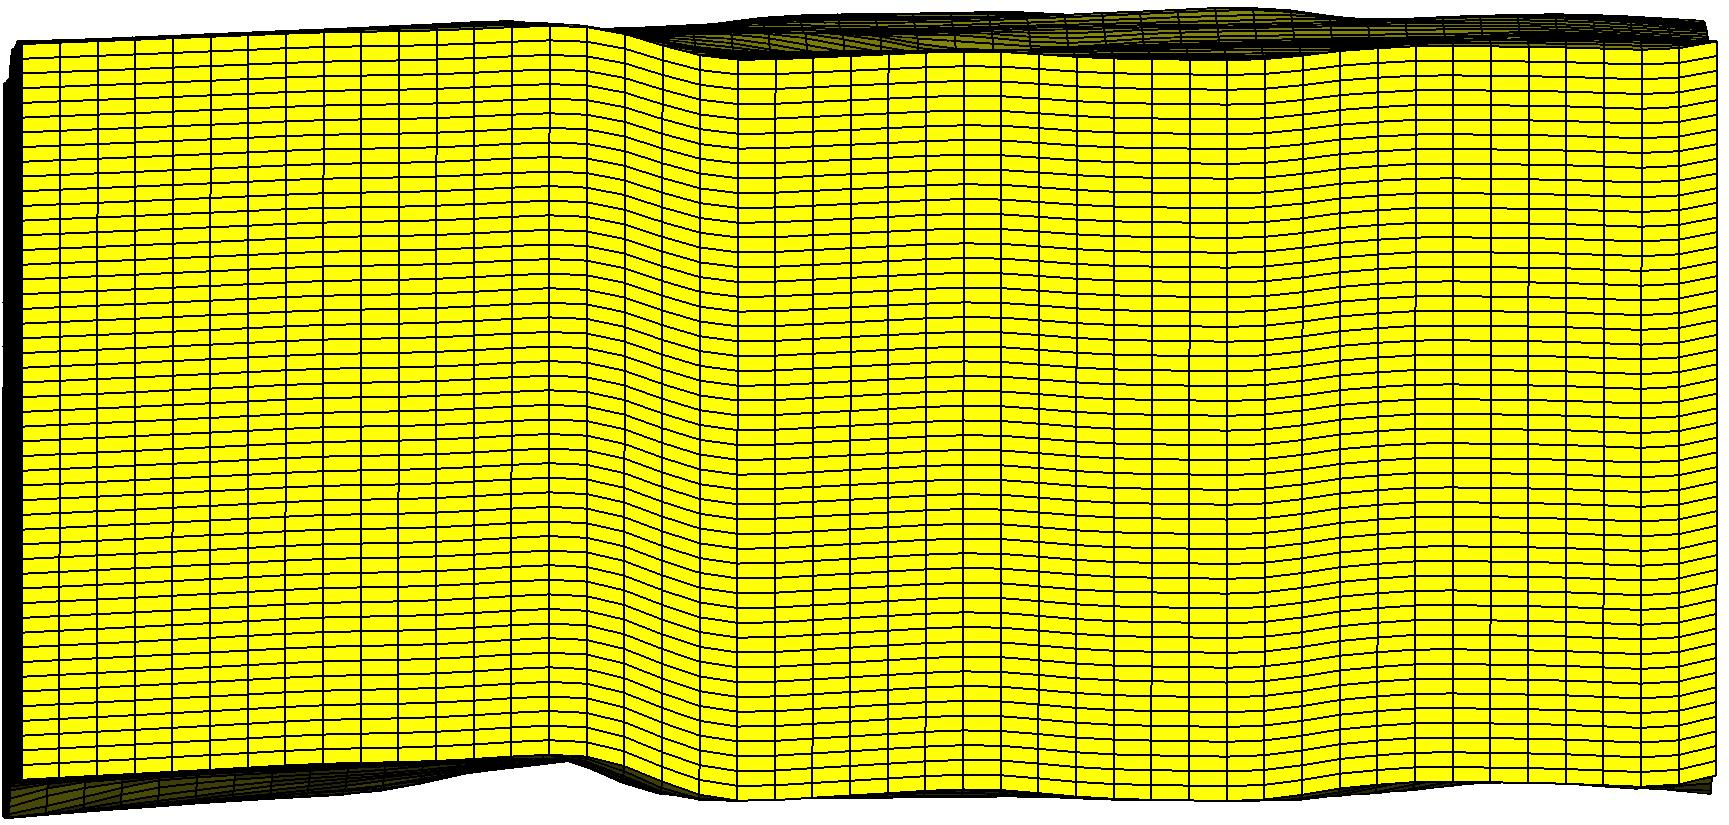
\includegraphics[width=.99\linewidth]{images/conformgrid}
%  \caption{The layer structure of a top- and base-conform grid.}
%  \label{fig:conformgrid}
%\end{figure}

\begin{figure}
  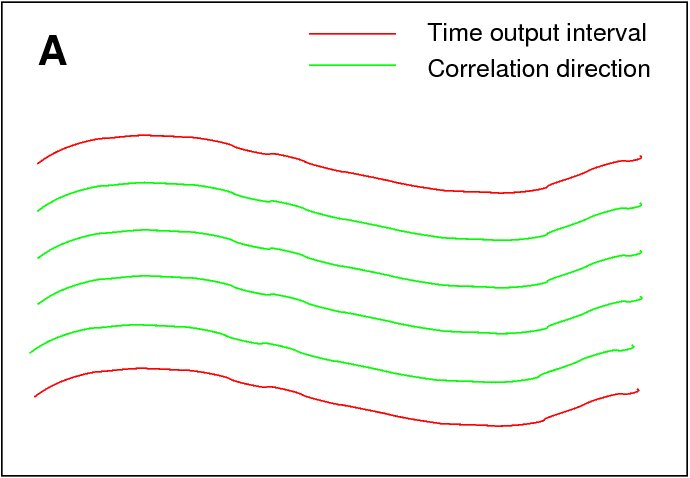
\includegraphics[width=.49\linewidth]{images/A_correlation_parallel}
  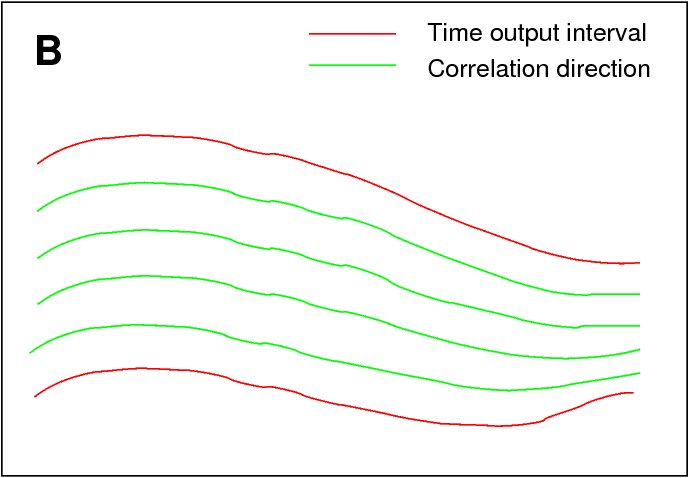
\includegraphics[width=.49\linewidth]{images/B_correlation_proportional}\\
  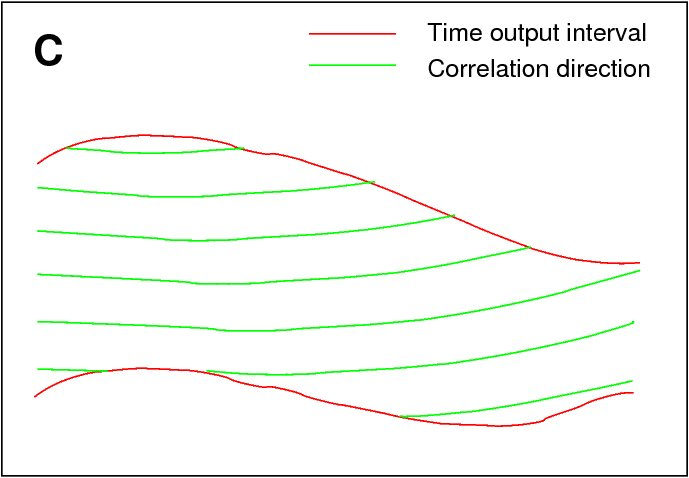
\includegraphics[width=.49\linewidth]{images/C_correlation_parallel_timecut}
  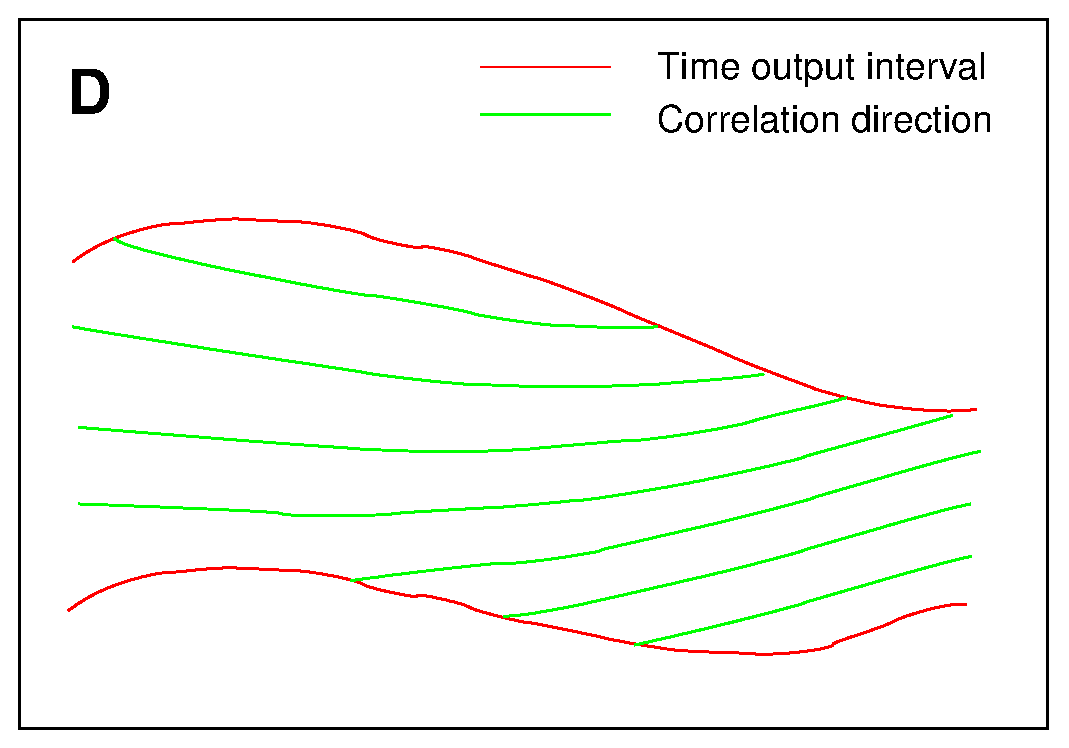
\includegraphics[width=.49\linewidth]{images/D_correlation_proportional_timecut}
  \caption{The layer structure of a (A) parallel top and base,
           (B) top- and base-conform compaction grid (C) Uniform correlation
           structure in a cut grid (D) Compactional correlation structure in a
           cut grid.} 
  \label{fig:inversion-interval-types}
\end{figure}

By specifying a correlation surface, the correlation direction can be
independent of the interval surfaces, see part C of
\autoref{fig:inversion-interval-types} and \autoref{sec:basiccorr}. If
this is done, there are no restrictions on the differences in interval
thickness.

The more flexible approach where a compactional correlation structure
is specified independent of the interval of interest (see part D of
\autoref{fig:inversion-interval-types})  is currently not implemented. 

If only one surface is known, the command \kw{interval-one-surface}
can be used to invert an interval with top and base parallel to this
surface. See \autoref{interval-one-surface} in the reference guide for
more details. Note that depth conversion and correlation surfaces will
not be available in this mode, so the lateral correlation will be
parallel to this surface, as illustrated in part A of
\autoref{fig:inversion-interval-types}. 

\subsubsection{Depth conversion}\label{sec:depthconvusr}
The \kw{output-volume} command is also where the depth conversion is
specified. Additional information for depth conversion has only to be
given under \kw{interval-two-surfaces}, since the lateral area is the
same. To do a depth conversion, one of the 
following must be given: 
\begin{itemize}
\item Reference surface in depth (either top or base), and a velocity cube.
\item Both top and base surface in depth. In this case, we assume constant velocity along each trace, computed from the time and depth surfaces.
\item Both top and base surface in depth, and a velocity cube. In this case, we use the cube for relative velocity in a trace, and scale it to match the interval length.
\end{itemize}

Reference surfaces in depth are given with the tags \kw{depth-file}\kwindex{depth-file} under \kw{top-surface} and/or \kw{base-surface}. The velocity cube can be read from file with the command \kw{velocity-field}\kwindex{velocity-field}. Alternatively, the command \kw{velocity-field-from-inversion}\kwindex{velocity-field-from-inversion} can be used to specify that \vp from inversion should be used for velocity. With depth conversion, the \kw{interval-two-surfaces} command may look like this:
\svex{ex:depthconv}
    <interval-two-surfaces>
      <top-surface>
        <time-file>      FlatTop_3100ms.storm </time-file>
        <depth-file>     FlatTop_3100ms.storm </depth-file>
      </top-surface>
      <base-surface>
        <time-file>      FlatBase_3600ms.storm </time-file>
        <depth-file>     FlatBase_3800ms.storm </depth-file>
      </base-surface>
      <velocity-field>   velocity.storm </velocity-field>
      <number-of-layers>            125 </number-of-layers>
    </interval-two-surfaces>
\end{verbatim}
\end{example}

\subsection{Prior model}
Since seismic data only contain information about relative elastic parameters, the absolute level needs to be set with a background model. In a Bayesian inversion setting, the background model is the prior expectation. We also need the prior covariance, which is given by the covariance of the parameters, the lateral correlation and the temporal correlation, as described in \autoref{sec:statmodthe}. In the model file, all this is gathered under the \kw{prior-model}\kwindex{prior-model} command, which may look something like this:
\svex{ex:priormodel}
<crava>
<prior-model>
  <background>
    <vp-file>      input/background/CravaBgVp.storm  </vp-file>
    <vs-file>      input/background/CravaBgVs.storm  </vs-file>
    <density-file> input/background/CravaBgRho.storm </density-file>
  </background>
  <lateral-correlation>
    <variogram-type> genexp </variogram-type>
    <power>       1 </power>
    <angle>       0 </angle>
    <range>    2500 </range>
    <subrange> 2500 </subrange>
  </lateral-correlation>
</prior-model>
</crava>
\end{verbatim}
\end{example}

\subsubsection{Background model}
\label{sec:basicbg}
The background model is given under the \kw{background}\kwindex{background} command. It can be given from file, using \kw{vp-file}\kwindex{vp-file}, \kw{vs-file}\kwindex{vs-file} and \kw{density-file}\kwindex{density-file}. These files should either be on Storm, crava, Sgri or SegY format. Alternatively, constant values can be used for background model, specified with \kw{vp-constant}\kwindex{vp-constant}, \kw{vs-constant}\kwindex{vs-constant} and \kw{density-constant}\kwindex{density-constant}. Any combinations of files and constants are also accepted. If none of these are given, the background model will be estimated.


Multiinterval (Multizone) background model is achieved by doing a \kw{multiple-intervals} inversion and with estimating background models activated. The surfaces are set under \kw{output-volume}.  It is not possible to  use multiinterval background with a single interval/zone inversion directly. To achieve this, one must first run Crava in estimation mode with \kw{multiple-intervals} and estimate a background model, where the written background model must then be used as input in a single interval inversion. The multiinterval background model will follow the other setting for multiinterval inversion, like \kw{correlation-direction}, \kw{erosion-priority} and \kw{uncertainty}. In each interval, a local background model is created by estimating a depth trend for the zone volume, then interpolating well logs into the depth trends using kriging. The full multiinterval background model is then made by joining the local background models in all the intervals.

\subsubsection{Covariances}
\label{sec:basiccorr}
As shown in \autoref{sec:statmodthe} the prior covariance structure for the elastic parameters consists of three parts:
\begin{enumerate}
\item A 3x3 covariance matrix for point-wise covariance between the parameters. May be read from ASCII file using the command \kw{parameter-correlation}\kwindex{parameter-correlation}.
\item A temporal correlation vector, length equal to number of layers in grid, $n_t$. May be read from ASCII file using the command \kw{temporal-correlation}\kwindex{temporal-correlation}.
\item A lateral correlation structure. May be given as a parametric variogram using the command \kw{lateral-correlation}.
\end{enumerate}
By default, the two first are estimated from well data, and the lateral correlation structure is set to a isotropic exponential variogram with range 1000. The reason for the latter choice is that this is hard to estimate, see \autoref{sec:correstimp} for details. The most common to override is the lateral correlation, where the variogram used for petro-physical modelling is a good choice.
\subsection{Well data}
Unless all information about wavelet, signal to noise and correlations are specified, well data are needed for estimation. Wells are given with the command \kw{well-data}\kwindex{well-data}, and may look like this:
\svex{ex:welldata}
<crava>
<well-data>
  <log-names>
    <time>    TWT  </time>
    <dt>      DT   </dt>
    <dts>     DTS  </dts>
    <density> RHOB </density>
  </log-names>
  <well>
    <file-name> input/logs/ed6406_3-3_cut.rms    </file-name>
  </well>
  <well>
    <file-name> input/logs/ed6506_12-3_cut.rms   </file-name>
  </well>
  <well>
    <file-name> input/logs/ed6506_12-8_cut.rms   </file-name>
  </well>
  <well>
    <file-name> input/logs/ed6506_12-S4H_cut.rms </file-name>
  </well>
</well-data>
</crava>
\end{verbatim}
\end{example}
There are two main elements here. The first is a well log
interpretation, given by \kw{log-names}, which tells \crava which
headers to look for. The following logs are needed: 
\begin{itemize}
\item Two way time log, specified with \kw{time}\kwindex{time}.
\item \vp log, either given by \kw{vp}\kwindex{vp} or \kw{dt}\kwindex{dt}. The latter is used for DT-logs.
\item \vs log, either given by \kw{vs}\kwindex{vs} or \kw{dts}\kwindex{dts}. The latter is used for DTS-logs.
\item Density log, given by \kw{density}\kwindex{density}.
\end{itemize}
In addition, if facies probabilities are computed, a facies log is
needed. This is specified with the tag \kw{facies}\kwindex{facies}. 

The wells are given with the command \kw{file-name} under
\kw{well}\kwindex{well}, which is given once for each well. The reason
for this is that additional information may be given for each
well. Well files should be on NORSAR or RMS-format. 

Each well may be moved to its optimal location using
\kw{optimize-position}\kwindex{optimize-location-to} under
\kw{well}\kwindex{well}, taking the arguments
\rkw{angle}{angle3}\kwindex{angle} and \kw{weight}\kwindex{weight}
which allow the user to assign different weights to the different
angle gathers for each well. The maximum allowed offset and vertical
shift for moving wells is specified in
\kw{maximum-offset}\kwindex{maximum-offset} and
\kw{maximum-shift}\kwindex{maximum-shift} under \kw{well-data}, with
default values of 250 m and 11 ms, respectively. 

The command \kw{synthetic-vs-log} tells whether the \vs log is
synthetic. If not specified, it will be detected from rank correlation
with \vp. The command
\kw{filter-elastic-logs}\kwindex{filter-elastic-logs} is used to do
multi-parameter-filtering of the elastic logs in this well after the
inversion. 

\subsection{I/O settings}
Two commands are used to specify the directory for input files. \kw{top-directory}\kwindex{top-directory} gives the working directory for the model file. 
The command \kw{input-directory}\kwindex{input-directory} is used to specify directory name for root directory for input files. The name is given relative to \kw{top-directory}.

Under \kw{advanced-settings}, the command
\kw{use-intermediate-disk-storage} can be used to limit the memory
usage when running large \crava jobs. A built-in smart-swap is then
activated. The option has largest effect on Microsoft Windows.

Under \kw{project-settings}, \kw{io-settings} and \kw{other-output}, the command \kw{error-file}\kwindex{error-file} writes all errors to a separate file, in addition to the log file. The command \kw{task-file}\kwindex{task-file} writes all tasks to a separate file, in addition to the log file. 
\subsection{Output}
Output is controlled under \kw{io-settings}\kwindex{io-settings} under
\kw{project-settings}. Here, you may set the output directory using
\kw{output-directory}\kwindex{output-directory}, and you may also
specify a prefix for all output files using
\kw{file-output-prefix}\kwindex{file-output-prefix}.

Except for the log file which is placed directly under the
output directory, all files output by crava are placed in
sub-directories. These sub-directories are 

\svex{ex:output-directories}
output-directory / wells 
                 / background 
                 / wavelets 
                 / seismic 
                 / velocity 
                 / correlations 
                 / inversionresults 
\end{verbatim}
\end{example}

There are two main output formats: Grid output, controlled by
\kw{grid-output}\kwindex{grid-output}, and well output controlled by
\kw{well-output}\kwindex{well-output}. The output section may look
something like this: 
\svex{ex:iosettings}
<crava>
<project-settings>
  <io-settings>
    <file-output-prefix> CRAVA_ </file-output-prefix>
      <grid-output>
        <format>
          <segy>       yes </segy>
        </format>
        <domain>
          <time>       yes </time>
          <depth>      yes </depth>
        </domain>
        <elastic-parameters>
          <vp>         yes </vp>
          <vs>         yes </vs>
          <density>    yes </density>
          <background> yes </background>
        </elastic-parameters>
      </grid-output>
      <well-output>
        <wells>         yes </wells>
        <blocked-wells> yes </blocked-wells>
      </well-output>
  </io-settings>
</project-settings>
</crava>
\end{verbatim}
\end{example}

\subsubsection{Grid output}\kwindex{grid-output}
Different elastic parameters can be given as grid output. In addition,
the estimated background model may be written as grids. This is
controlled by the \kw{elastic-parameters}\kwindex{elastic-parameters}
command under \kw{grid-output}. See \autoref{elastic-parameters} for a
full list of possible grids. If this command is not used, \vp, \vs and
density will be written. Output of original and synthetic seismic data
can be given by the \kw{seismic-data}\kwindex{seismic-data}
command. Other grids can be requested for output by the command
\kw{other-parameters}\kwindex{other-parameters}, for example
correlations. 

The grid format may be controlled using \kw{format}\kwindex{format}. Here the yes/no parameters \kw{storm}, \kw{segy}, \kw{sgri}, \kw{crava} and \kw{ascii} can be used to decide if grids should be written on storm- (RMS), segy-, Sgri-, crava- or ASCII-format. You may choose several formats for one run; all grids will be written on all selected formats. The Segy format can be controlled by the \kw{segy-format} command, in the same way as for input data, described in \autoref{sec:basicseis}. Note that correlation grids make sense only in storm format. Default output format is storm. The crava format is a binary format only to be used with \crava. It can be read and written from \crava, and is useful if the output from a \crava run should be used as input to another \crava run because the format is fast to read.

By using the \kw{domain}\kwindex{domain} option, output may be written
in time domain \kw{time} or depth domain \kw{depth} (requires
parameters set under \kw{output-volume}, see
\autoref{sec:depthconvusr}), or both. Again, correlation grids only
make sense in time domain, which is default. 

\subsubsection{Well output}\kwindex{well-output}
Some versions of filtered elastic parameters (\vp, \vs and density) in wells can be generated by the \kw{well-output} command. The wells can be given in two different formats, RMS or NORSAR. This is controlled by the \kw{format}\kwindex{format} command. The logs written are
\begin{itemize}
\item Raw elastic logs.
\item Elastic logs filtered to background frequency.
\item Elastic logs filtered to seismic frequency.
\item Elastic logs filtered with facies prediction filter (if available).
\item Facies log (if available).
\end{itemize}
The wells can either be written with original sampling density, using \kw{wells}, or matching the internal grid resolution, using \kw{blocked-wells}.

\subsection{Actions}
The final information that is needed for a \crava run is what the run is supposed to do. This is controlled by \kw{actions}\kwindex{actions}. The \kw{mode} keyword defines the purpose of this run and should be set to "inversion" when doing inversion. Other options are "estimation", see \autoref{sec:estimateusr} and "forward", see \autoref{sec:forwardusr}. When inversion is chosen, \kw{inversion-settings}\kwindex{inversion-settings} can be used to control basic aspects of the inversion. It may look something like this:
\svex{ex:action}
<crava>
<actions>
  <mode>                    inversion </mode>
  <inversion-settings>
    <prediction>                  yes </prediction>
    <simulation>
      <seed>                   150570 </seed>
      <number-of-simulations>      10 </number-of-simulations>
    </simulation>
  </inversion-settings>
</actions>
</crava>
\end{verbatim}
\end{example}

The command \kw{prediction}\kwindex{prediction} can be used to turn
predictions on or off. By default, the prediction will be generated. A
number of full frequency stochastic realisations of the inversion can
be obtained by specifying \kw{number-of-simulations}\kwindex{number-of-simulations} under \kw{simulation}\kwindex{simulation}. The seed for the random generator can also be given here, with the \kw{seed}\kwindex{seed} command. Changing the seed will give a new set of realisations.

The command \kw{kriging-to-wells}\kwindex{kriging-to-wells} can be
used to krige realisations to well data. By default, this is done if
the \kw{simulation} command is used. 

\subsection{Standard formats for input and output}
\label{sec:gridformats}

\subsubsection{3D-grid}
Crava can read and write the following 3D grid
  formats: SegY, Storm, Sgri (NORSAR) and crava (internal) . On
  output, the format is controlled by a \kw{format} keyword. On input,
  the program automatically detects the format, although it may need
  help to correctly read SegY formats, using the \kw{segy-format}
  keyword. The default output format is storm.

\subsubsection{Surfaces}
The standard format for reading and writing
  surfaces is binary storm, but \crava can also read Roxar ASCII
  surfaces (formerly known as ASCII Irap classic), Multicolumn ASCII
  surfaces (see example below) and XYZ ASCII surfaces. Multicolumn ASCII and XYZ ASCII files must follow the segy geometry.
   In addition some surfaces related to 3D-inversion are read as sgri (NORSAR). On input,
  the surface format will be automatically detected. For writing we currently support Roxar Ascii and Storm binary.
  
\paragraph{Multicolumn Ascii example}
The multicolumn ascii file is a text file with five columns, and each columns needs ta have a header name:
X or UTMX; Y or UTMY; IL or Inline; XL or Crossline; Z, TWT or Attribute. The order of the columns is arbitrary. The file might also have some text before the header-row. This surface is based segy-geometry and must follow the corresponding seismic cube, as the reference point, angle and area are taken from the geometry. We require even sampling in the file, but we do not require as fine sampling as in the seismic. It is for example possible to give only the four corners of the surface. A segy geometry will be required for using multicolumn ascii files. The standard missing value is defined as $-999.25$.

A file may look like:
\begin{table}[h]
\centering
\label{tab:multicolumnascii}
\begin{tabular}{lllll}

X         &         Y              &     Inline       &   Crossline     &    Attribute\\ 
455380.0    &        6799690.0   &        2100.0      &       5600.0       &       2467.05737 \\ 
447256.0    &        6799789.0    &       2100.0       &       5640.0      &        2480.06712\\ 
447393.0    &        6811038.5     &      2120.0      &        5600.0      &        2549.43453\\ 
455517.0    &        6810939.5     &      2120.0      &        5640.0      &        2338.12905\\ 
\end{tabular}
\end{table}

\paragraph{XYZ Ascii example}
The xyz ascii file is a text file with three columns, X, Y and Z. The columns may have a header name, X or UTMX; Y or UTMY; Z, TWT or Attribute. Columns may also be given in an arbitrary order. If there is no header line, it is assumed that the order is x, y, z. This surface is based segy-geometry and must follow the corresponding seismic cube. We require even sampling in the file, but we do not require as fine sampling as in the seismic. It is for example possible to give only the four corners of the surface. A segy geometry will be required for using xyz ascii files. The standard missing value is defined as $-999.25$.

A file may look like:
\begin{table}[h]
\centering
\label{tab:xyzascii}
\begin{tabular}{lll}

X         &         Y              &    Z\\ 
455380.0    &        6799690.0   &        2467.05737 \\ 
447256.0    &        6799789.0    &       2480.06712\\ 
447393.0    &        6811038.5     &      2549.43453\\ 
455517.0    &        6810939.5     &      2338.12905\\ 
\end{tabular}
\end{table}


\subsubsection{Wavelets}
Wavelets are either on JASON or NORSAR format,
  both for reading and writing. Auto-detect is used on reading, use \kw{format3}
  for writing. The default output format is JASON.

\subsubsection{Wells}
For reading we support wells on RMS, NORSAR and LAS format. For writing we currently support RMS and NORSAR. Auto-detect is used on reading; use \kw{format2} to control writing. The default output format is RMS.

\section{Advanced inversion options}
\label{sec:advinvusr}
Although \crava is mainly intended as a simple and fast inversion
tool, there are still some options to control the inversion, and to
access more sophisticated approaches. Most of these are covered here,
see 
also \autoref{advanced-settings} for details about
\kw{advanced-settings}. 
\subsection{Non-stationary wavelet and noise}
Although the FFT-algorithm which is at the core of \crava requires
stationarity, this does not mean that the entire inversion has to be
stationary, as discussed in \autoref{sec:nonstationaryimp}. We allow
lateral variations in wavelet amplitude, wavelet shift and signal to
noise ratio.

The local wavelet transformations fit well within the core framework
of \crava, but the local noise requires some approximations, as
explained in section \autoref{sec:localnoiseimp}. This means that
local noise only improves the final result if the local variations are
substantial. We do not recommend using local noise if the variation in
noise level is less than 15\%.

Unlike the basic level, where parameters that were not specified 
automatically got estimated, the use of local wavelets or local noise
must be explicitly triggered. For wavelets, this is done with the
\kw{local-wavelet}\kwindex{local-wavelet} command under
\kw{wavelet}. There are four alternatives:
\kw{local-wavelet}: 
\begin{enumerate}
\item \kw{shift-file} gives a file name for a map giving the local shifts. 
\item \kw{estimate-shift} will estimate a local shift map when set to "yes".
\item \kw{scale-file} gives a file name for a map giving the local scale. 
\item \kw{estimate-scale} will estimate a local scale map when set to "yes".
\end{enumerate}
Naturally, the shift can not be both given and estimated, the same
holds for scale. Note that you may choose to use only shifts, omitting
both scale keywords, or use only scale. 

The local noise is triggered similarly, by using one of two
commands under \kw{angle-gather}: 
\begin{enumerate}
\item \kw{local-noise-scaled} gives a file name for a map with the local scaling of
  the signal to noise ratio.
\item \kw{estimate-local-noise} estimates the local scaling of the
  signal to noise ratio if set to "yes". 
\end{enumerate}

\subsection{PS-seismic and reflection approximations}
By default, \crava assumes that the input seismic data are PP, but PS
data can also be used. For both cases, we use the linearised
Aki-Richards approximation, see \autoref{eq:aki_c}. The type of seismic data is
indicated by using the \kw{type}\kwindex{type} command
under\kw{seismic-data}. Here, \kw{type} should be either "pp" or
"ps". Note that PS data must also be aligned in PP-travel time, as no
such alignment is done internally by \crava. 

Instead of using the default reflection approximation, the user may
supply the parameters to compute the reflections. We always assume
that for a given angle and seismic type, the reflections can be
computed from the equation 
\begin{equation}
\begin{split}
  c(\vect{x},t,\theta)
  & = a_{V\!p} (\theta) \frac{\partial}{\partial t}\ln\vp (\vect{x},t)\\
  & + a_{V\!s} (\vect{x},t,\theta) \frac{\partial}{\partial t}\ln\vs (\vect{x},t)\\
  & + a_\rho(\vect{x},t,\theta) \frac{\partial}{\partial t}\ln\rho(\vect{x},t).
\label{eq:linrefl}
\end{split}
\end{equation}
The coefficients $a_{V\!p}$, $a_{V\!s}$ and $a_\rho$ can be read from
file, using the \kw{reflection-matrix}\kwindex{reflection-matrix}
command under \kw{advanced-settings}. This file should have one line
for each seismic data file, and each line should have the three
coefficients for one set of seismic input data. The order of the lines
should be the same as the order of the seismic data in the \kw{survey}
command. 

\subsection{Well quality checks}
Well logs are often faulty, and \crava has some safety mechanisms to
detect this. The primary mechanism is to detect extreme values, and
set these undefined. The default upper and lower bounds accepted in
well logs are shown in \autoref{tab:logminmax}. These can be
overridden using the command 
\kw{allowed-parameter-values}\kwindex{allowed-parameter-values} under
\kw{well-data}. Here, \kw{minimum-vp}, \kw{minimum-vs},
\kw{minimum-density} and the corresponding maximum values can be
given. 
\begin{table}
\caption{Default intervals for valid well log values.\label{tab:logminmax}}
\begin{tabular}{|lrr|}
\hline
& Min & Max \\
\hline
\vp & 1300 & 7000 \\
\vs &  200 & 4200 \\
$\rho$ & 1.4 & 3.3 \\
\hline
\end{tabular}
\end{table}

Some logs may stay within reasonable values, but have too much or too
little variation, also indicating that something is wrong. We
therefore calculate the variance of the logarithm of the log minus the
background, and if this is outside reasonable bounds, an error is
triggered. The default bounds shown in \autoref{tab:logvarminmax} can
be overridden with \kw{allowed-parameter-values}, using
\kw{minimum-variance-vp}, and so forth. 
\begin{table}
\caption{Default intervals for valid well log variances.\label{tab:logvarminmax}}
\begin{tabular}{|lrr|}
\hline
& Min & Max \\
\hline
Var(ln(\vp)) & $5*10^{-4}$ & $250*10^{-4}$ \\
Var(ln(\vs)) & $10*10^{-4}$ & $500*10^{-4}$ \\
Var(ln($\rho$)) & $2*10^{-4}$ & $100*10^{-4}$ \\
\hline
\end{tabular}
\end{table}

\subsection{Generate synthetic seismic from inversion data}
It is possible to generate synthetic seismic by a forward modelling
with the \vp, \vs and density resulting from the inversion. This is done
by the command  \kw{synthetic} under \kw{seismic-data} under
\kw{grid-output}, \kw{io-settings},  in command
\kw{project-settings}. 

\section{Estimation}
\label{sec:estimateusr}
As mentioned, \crava can estimate many of the needed parameters. There
are several commands that control the estimation behaviour for
wavelets, noise and background model. Note that the correlations will
always be estimated as explained in \autoref{sec:correstimp} from all
available well logs, and do not have any further controls. 

\subsection{Estimation mode}
If you only want to do the estimation, in order to check the quality
of the estimates, you can use "estimate" in the \kw{mode}
command. Using this, \crava will perform the initial model building
tasks and estimate needed information, but terminate once all
information needed for inversion is estimated. When running in
estimation mode, you can also control the main estimation aspects
using the \kw{estimation-settings}\kwindex{estimation-settings}
command. This allows you to control which of the main estimation tasks
should be carried out, setting yes or no for
\kw{estimate-correlations}, \kw{estimate-wavelet-or-noise} or
\kw{estimate-background}. Parameters with a "no" will not be estimated
unless needed for other estimations. Note that in estimation mode, all
estimated parameters are written to file, regardless of output
settings. 
\subsection{Wavelet and noise estimation}
Wavelets and noise are estimated together. These parameters will only
be estimated from wells that are vertical or close to vertical, since
this allows comparing synthetic seismic from well logs with one or a
couple of traces, and thus reduces alignment issues. The angle limit
can be controlled by the
\kw{maximum-deviation-angle}\kwindex{maximum-deviation-angle} command
under \kw{well-data}. In addition, wells can be excluded individually,
by setting \kw{use-for-wavelet-estimation} to "no" under \kw{well}. 

By default, the wavelet and noise are estimated in the region between
the top and base surface for the inversion area. This may be limited
using the \kw{wavelet-estimation-interval} command under 
\kw{survey}, where a separate set of restricting surfaces are given
with \rkw{top-surface}{top-surface3}, \rkw{time-file}{time-file3} and 
\rkw{base-surface}{base-surface3}, \rkw{time-file}{time-file3}. It is
also possible to specify these restrictions a contant value, using
the \rkw{time-value}{time-value3} keyword. Since these are
under \kw{wavelet}, they can be different for each angle. 

Some wavelet estimation options are also found under the command
\kw{advanced-settings} given under \kw{project-settings}. These are 
\begin{itemize}
\item \kw{wavelet-tapering-length} which controls the length of the wavelet (in ms).
\item \kw{minimum-relative-wavelet-amplitude} which finds the wavelet
  length, by setting the cutoff size for edge peaks relative to centre
  peak. 
\item \kw{maximum-wavelet-shift} which controls how far the wavelet
  can be shifted locally, see \autoref{sec:waveestimp}. 
\end{itemize}

Prior information for local wavelet modelling is given by the
\kw{local-wavelet} command under \kw{prior-model}. Here, lateral
correlation is specified as  a 2D variogram for the lateral
correlation in local wavelet modelling by the command
\kw{lateral-correlation}. 

Output of wavelets is controlled by the \kw{wavelet-output}\kwindex{wavelet-output} command under \kw{io-settings}. 
Two different formats can be specified, JASON and NORSAR. Estimated wavelets for each well is written by the 
\kw{well-wavelets}\kwindex{well-wavelets} command. The command \kw{global-wavelets}\kwindex{global-wavelets} 
writes global wavelets for each seismic angle. If local wavelet is requested, the command 
\kw{local-wavelets}\kwindex{local-wavelets} writes estimated local wavelet shift and scale surfaces.

Output of estimated local noise surface is given by the command
\kw{local-noise} given under \kw{io-settings} and \kw{other-output}. 

\subsection{Background model estimation}
The background model is estimated as a low frequency vertical
trend. The trend is given in relative depth in the inversion volume,
so the trend value along the top and base surface is constant. At
well locations, the trend is kriged to the well logs. By default, all
wells are used for background model estimation, but can be excluded by 
specifying "no" for \kw{use-for-background-trend} under \kw{well} for individual
wells. 

The background estimation can be controlled by some commands under
\kw{background}\kwindex{background}. These are: 
\begin{itemize}
\item \kw{velocity-field} takes an external velocity field, typically
  from migration, and uses as \vp background, kriged to low frequency
  \vp well logs. 
\item \kw{lateral-correlation} gives a variogram for the
  kriging. Larger ranges extends the influence of well data further
  away from wells. 
\item \kw{high-cut} allows specification of a maximum frequency for
  the background model. 
\end{itemize}

\subsection{Prior correlations}
Prior correlations between \vp, \vs and density, and autocorrelation are estimated. they can be written to file by the command \kw{prior-correlations}\kwindex{prior-correlations} under \kw{project-settings}, \kw{io-settings} and \kw{other-output}.

\section{3D wavelet}
Instead of the traditional 1D wavelet a 3D wavelet can be used in
\crava. This wavelet is constructed by a 1D pulse and a 3D wavelet
filter based on illumination vectors. The use of a 3D wavelet is
invoked by the keyword \kw{wavelet-3d}.  

The 1D pulse used to construct the 3D wavelet, can be specified by the
\kw{file-name} keyword. If a file is not specified, this pulse is
estimated. Either way, a filter file must be given by the keyword
\kw{processing-factor-file-name}. This filter contains the amplitude
effects related to the illumination vectors and is given on Sgri
format. One or two filters are given. The first, and necessary,
contains frequency-independent amplitude effects, while the second, if
given, contains frequency-dependent amplitude effects. 

For noise estimation in the 3D wavelet setting, a propagation filter
file is given by the keyword \kw{propagation-factor-file-name}. At
present, this is not used. The keyword \kw{stretch-factor} can be
given, but is not used since the stretch factor is automatically
calculated from the offset angle. 

When estimating the 1D pulse, seismic data from a neighbourhood of the
well can be used. The distance from the well, specified in meters,
that data are collected is given by the commands
\kw{estimation-range-x-direction} and
\kw{estimation-range-y-direction}. The default is that only data from
the well position are used.   

When 3D wavelet is used, certain parameters related to the mapping
between time and depth are needed. This occurs since the illumination
vectors relates to depth, while \crava works in time. These
settings are given under keyword
\kw{time-to-depth-mapping-for-3d-wavelet} in \kw{project-settings}. A 
reference depth for the target area must be specified under the keyword
\kw{reference-depth}. This depth represents a constant surface which 
in time normally will refer to a variable surface due to varying
velocity above this depth. This reference surface is given by
\kw{reference-time-surface} and can be given on Storm- or
Sgri-format. The parameter \kw{average-velocity} refers to the average
velocity in the target area which is needed for the estimation of the
pulse.  

\section{Rock physics}
\label{sec:rockPhysics}
The idea behind the rock physics template is to be able to model the density and elastic properties of a fluid-filled \kw{rock} in a very flexible way, by selecting from and possibly combining many different rock physics theories. In order to do this, we need some basic building blocks. The basic building blocks here are \kw{fluid}, \kw{solid}, \kw{dry-rock} (a solid with porosity, but no fluid) and \kw{rock} (a combination of solid and fluid).

In \crava, the rock physics models are used for generating the background model and covariance matrix used in the prior model, and for generating synthetic wells used for facies estimation. 

\subsection{Structure of the rock physics template}
The base structure of the rock physics template consists of the elements \kw{reservoir}, \kw{evolve}, \kw{predefinition}, \kw{rock} and \kw{trend-cube}, each of which contains sub-elements.

The sub-elements will be basic building blocks (e.g. \kw{solid}, \kw{fluid}, \kw{dry-rock}), properties (e.g. temperature, pore-pressure, density, etc) and theories.

\subsubsection{Reservoir}
\kw{reservoir} contains reservoir properties, such as pressure, temperature, porosity, fluid saturation, lithology, etc. Reservoir properties given under the keyword \kw{reservoir} are parameters common for fluids, solids, dry rocks and rocks. For models that depend on these parameters, the values given under reservoir can be used, although they may be overridden locally. The elements in \kw{reservoir} are defined by labels to be referred to with the \kw{reservoir-variable} statement. Hence, they must be unique. 
After \kw{reservoir}, the command \kw{variable} follows. Below is an example of how \kw{reservoir} can be defined:
\svex{ex:Reservoir}
<reservoir>
  <variable>
    <label> temperature </label>
    <value> 50 </value>
  </variable>

  <variable>
    <label> porosity </label>
    <gaussian>
      <mean> 0.5 </mean>
      <variance> 0.1 </variance>
    </gaussian>
  </variable>
</reservoir>
\end{verbatim}
\end{example}

\subsubsection{Evolve}
\kw{evolve} controls the time development of the reservoir variables. Under the keyword \kw{evolve}, \rkw{reservoir-variable}{reservoir-variable-evolve}, \kw{one-year-correlation} and \rkw{vintage}{vintage-evolve} are given. \kw{reservoir-variable} needs to be the label of one of the variables defined in \kw{reservoir}. \kw{one-year-correlation} defines the correlation between the reservoir variable at two following years. \rkw{vintage}{vintage-evolve} is repeated for each vintage of the time development. In \rkw{vintage}{vintage-evolve}, \rkw{distribution}{distribution-vintage} and \kw{vintage-year} are given. \rkw{distribution}{distribution-vintage} is the distribution of the reservoir variable at the given vintage, and it needs to be one of the distributions given under \kw{value-assignments}. \kw{vintage-year} is the year of the given vintage of the reservoir variable.
Below is an example with \kw{evolve} for the reservoir variable porosity:
\svex{ex:evolve}
<evolve>
  <reservoir-variable> porosity </reservoir-variable>
  <one-year-correlation> 0.7 </one-year-correlation>
  <vintage>
    <distribution>
      <beta>
        <mean> 0.1 </mean>
        <variance> 0.01 </variance>
      </beta>
    </distribution>
    <vintage-year> 2000 </vintage-year>
  </vintage>

  <vintage>
    <distribution>
      <beta>
        <mean> 0.08 </mean>
        <variance> 0.01 </variance>
      </beta>
    </distribution>
    <vintage-year> 2002 </vintage-year>
  </vintage>
</evolve>
\end{verbatim}
\end{example}

\subsubsection{Predefinitions}
\kw{predefinitions} is used for specifying and calculating the elastic properties of basic building blocks, being \kw{solid}, \kw{fluid} or \kw{dry-rock}, or elements and mixtures of these. It will typically use properties specified under \kw{reservoir}. 

Each time a building block is defined, it is given a unique identifying name using the \kw{label} keyword. This is followed by a keyword specifying which theory we use for building this element, and inside that keyword block, the required parameters for the theory are given. 

Inside the theory block, the required parameters for the theory are given. 
The theories are used for calculating the bulk and shear moduli. In addition, they are implicitly used for calculating the density using the arithmetic average of the constituent densities. 

If we want to use an element that is already defined, we can use the keyword \kw{use} instead of \kw{label}, followed by the unique name of the element. Thus, we can easily reuse elements once they are defined.

The significant difference between elements in \kw{reservoir} and \kw{predefinitions} is that each element in \kw{reservoir} defines a single property, while it defines an object with several properties in \kw{predefinitions} (e.g. bulk modulus, shear modulus and density). These objects are typically used as inputs to various theories for calculating the effective properties of a mixed material.

\svex{ex:predefinitions}
<predefinitions>
  <solid>
    <label> quartz </label>
    <tabulated>
      <bulk-modulus> 37 </bulk-modulus>
      <shear-modulus> 44 </shear-modulus>
      <density> 2.65 </density>
    </tabulated>
  </solid>
  <fluid>
    <label> brine </label>
    <batzle-wang-brine>
      <pore-pressure> 20 </pore-pressure>
      <temperature> 60 </temperature>
      <salinity> 0.05 </salinity>
    </batzle-wang-brine>
  </fluid>
</predefinitions>
\end{verbatim}
\end{example}

\subsubsection{Rock}
\kw{rock} contains the final composition of the rock, and will typically use details specified in \kw{reservoir} and \kw{predefinitions}. The \kw{rock} command is followed by either \kw{label} or \kw{use}. If \kw{label} is used, the next keyword is a theory. 

The rocks to be used in the facies estimation, need to correspond to the facies given in \kw{facies-probabilities}.

Example:

\svex{ex:rock}
<rock>
  <label> effective rock </label>
  <gassmann>
    <dry-rock>
      <use> quality sand </use>
    </dry-rock>
    <fluid>
      <use> brine </use>
    </fluid>
  </gassmann>
</rock>
\end{verbatim}
\end{example}

\subsubsection{Trend cubes}
<trend-cube> contains the trend cubes that can be used for defining a trend on the variables. Each variable defined by a trend may be related to one or two trend cubes. These trend cubes may for example be related to time and depth, and they need to be defined in the entire inversion volume. 

\subsection{Value assignments in the rock physics template}
All the properties and function parameters can use previously assigned values defined in <reservoir>, or be assigned values directly in <predefinitions>. The possible types of value assignments are value, trend or distribution. 

\subsubsection{Value}
The simplest form of deterministic value assignment is a single value. For the variables in <reservoir>, the value is given by the command <value>, while it may be given directly for the variable commands of <predefinitions>. Below is an example for each of these cases:
\svex{ex:assignValue}
<reservoir>
  <variable> 
    <label> temperature </label>
    <value> 40 </value>
  </variable>
</reservoir>

<predefinitions>
  <solid>
    <label> clay </label>
    <tabulated>
      <bulk-modulus> 21 </bulk-modulus>
      <shear-modulus> 7 </shear-modulus>
      <density> 2.6 </density>
    </tabulated>
  </solid>
</predefinitions>
\end{verbatim}
\end{example}

\subsubsection{Distributions}
The rock physics template supports the distribution functions \kw{gaussian}, \kw{beta} and \kw{beta-end-mass} for assigning probabilistic values to a variable. Whenever several building blocks use the same stochastic variable defined under <reservoir>, the same sample of the variable is used for all the building blocks. The required input variables for the different distributions are given in \autoref{sec:valueassignment}.

Examples:
\svex{ex:assignDistribution}
<reservoir>
  <variable>
    <label> total-porosity </label>
    <gaussian>
      <mean> 0.25 </mean>
      <variance> 0.05 </variance>
    </gaussian>
  </variable>

  <variable>
    <label> bulk-quartz </label>
    <beta>
      <mean> 63000000 </mean>
      <variance> 30000 </variance>
      <lower-limit> 10000000 </lower-limit>
      <upper-limit>100000000</upper-limit>
    </beta>
  </variable>
</reservoir>
\end{verbatim}
\end{example}

\subsubsection{Assigning trends to the rock physics variables}
\label{sec:assigntrendsrockphy}
The values of the variables may be given by a trend. The trends are named \kw{trend-1d} or \kw{trend-2d}, with the 1d and 2d endings telling if the property values should be related to one or two trend cubes. These trend cubes may for example be related to time and depth, and they need to be defined in the entire inversion volume. If the trend is to be used, trend cubes must be given on the same level as \kw{reservoir} using the command \kw{trend-cube} following the example below. 
If the trend represent a mean or a variance (as in for example the background model), these can be estimated from data by specifying either \kw{mean} or \kw{variance} in  addition to using the command \kw{estimate}. Note that if the model is 1-dimensional, it is necessary to specify the reference parameter, see the examples below. The estimation methods are version of standard kernel smoothing (local linear regression for the mean and a weighted kernel smoothing for the variance). Note that the mean and variance does not need to have the same dimensionality, see the examples below.


\svex{ex:assignTrend}
<reservoir>
  <variable> 
    <label> temperature </label>
    <trend-1d>
      <file-name> trend1d.txt </file-name>
      <reference-parameter> time </reference-parameter>
    </trend-1d>
  </variable>

  <variable> 
    <label> porosity </label>
    <trend-2d> 
      <file-name> trend2d.txt </file-name>
      <reference-parameter-first-axis> time 
      </reference-parameter-first-axis>
      <reference-parameter-second-axis> depth 
      </reference-parameter-second-axis>
    </trend-2d>
  </variable>
</reservoir>

<trend-cube>
  <parameter-name> time </parameter-name>
  <file-name> trendCubeTime.txt </file-name>
</trend-cube>

<trend-cube>
  <parameter-name> depth </parameter-name>
  <file-name> trendCubeDepth.txt </file-name>
</trend-cube>

<vp>
  <gaussian>
    <mean>
      <trend-2d>
        <estimate>yes</estimate>
      </trend-2d>
    </mean>
    <variance>
      <trend-1d>
       <estimate>yes</estimate>
        <reference-parameter>twt</reference-parameter>
      </trend-1d>
    </variance>
  </gaussian>
</vp>

<vp>
  <gaussian>
    <mean>
      <trend-1d>
        <estimate>yes</estimate>
        <reference-parameter>twt</reference-parameter>
      </trend-1d>    
    </mean>
    <variance>
      <estimate>yes</estimate>      
    </variance>
  </gaussian>
</vp>

\end{verbatim}
\end{example}


\section{Facies prediction}
An important feature in \crava is the ability to create facies
probabilities. This requires that \kw{mode} is set to "inversion", and
is triggered by the \kw{facies-probabilities} command under
\kw{inversion-settings}. 
%The value given here should be either
%"absolute" or "relative", corresponding to probability computations
%based on absolute or relative inverted parameters. 


The facies probabilities are computed based on the inversion results
and a distribution for inversion values given facies computed from
filtered well logs, where the filter is defined by the inversion. See
\autoref{sec:facprobthe}. Probability volumes will be computed for all
facies seen in wells, and if the command
\kw{facies-probabilities-with-undef}\kwindex{facies-probabilities-with-undef}
is used, an additional undefined probability cube is
also generated, indicating areas where the inversion values are too
far away from well data to make reliable predictions. 

Except from the trigger in \kw{inversion-settings}, all parameters
related to facies probabilities are given under
\kw{facies-probabilities}\kwindex{facies-probabilities} under
\kw{prior-model}. Here is an example: 
\svex{ex:facprob}
<crava>
<prior-model>
  <facies-probabilities>
    <use-vs>                          yes </use-vs>
    <use-prediction>                  yes </use-prediction>
    <use-absolute-elastic-parameters> yes </use-absolute-elastic-parameters>
    <estimation-interval>
      <top-surface-file>  input/horizons/facies_top.storm  </top-surface-file>
      <base-surface-file> input/horizons/facies_base.storm </base-surface-file>
    </estimation-interval>
    <prior-probabilities>
      <facies>
        <name>          sand </name>
        <probability>    0.4 </probability>
      </facies>
      <facies>
        <name>         shale </name>
        <probability>    0.6 </probability>
      </facies>
    </prior-probabilities>
  </facies-probabilities>
</prior-model>
</crava>
\end{verbatim}
\end{example}

\begin{figure}[h]
  \centering
  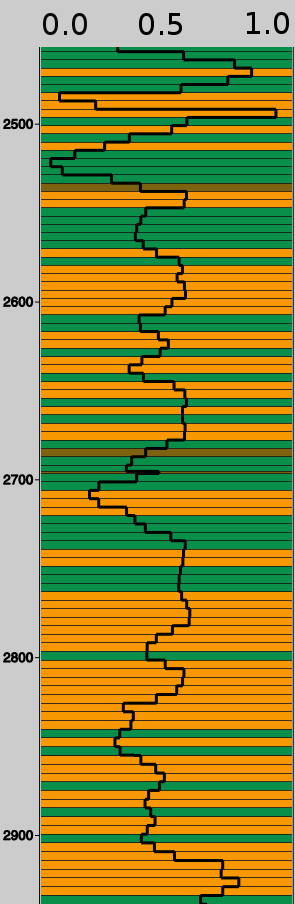
\includegraphics[width=.305\linewidth, height=100mm]{images/sand_probability_well_off}\qquad
  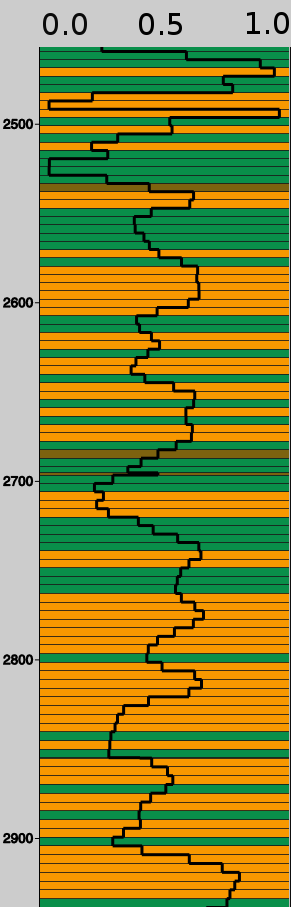
\includegraphics[width=.300\linewidth, height=100mm]{images/sand_probability_well_on}
  \caption{A sample facies probability estimation. The black curve gives the
    probability of sand in a well containing sand (orange), shale
    (green) and crevasse (brown). In the left figure the well was not
    included in the facies probability estimate whereas it was
    included in the right figure.} 
  \label{fig:sandprob}
\end{figure} 

If \kw{use-absolute-elastic-parameters} is set to 'yes', facies probability is computed based on
inverted parameters including background model.
If the distribution
for elastic parameters for each facies is constant over the inversion
volume, using absolute values is more stable. However, if there are
trends in the elastic parameters, the relative values are more
robust. The default is to use relative values.

%Instead of \kw{probability}, we can use \kw{probability-cube}, where
%prior facies probabilities are given on a file. A prior value for
%undefined facies is set with the command \kw{uncertainty-level}. 

The interval to use for facies probability calculations can be
set with \kw{estimation-interval}, similar to
estimation interval for wavelets. Parallel to the wavelet case, wells
may also be excluded using the \kw{use-for-facies-probabilities}
command under \kw{well}.

\subsection{Prior probabilities}
In order to get reliable probabilities, we need good prior
probabilities. By default, \crava computes the average fraction of
each facies in the relevant interval of the wells. This can be
overridden using the \kw{prior-probabilities} command, which
allows specification of these. Note that probabilities must be given
for each facies. Probabilities can either be given globally, with
\kw{probability}, or as a full 3D trend, using
\kw{probability-cube}. The latter takes a grid file as argument,
and the corresponding grid must cover the inversion volume.
A prior value for
undefined facies is set with the command \kw{uncertainty-level}. 

\subsection{Output parameters}
Facies probabilities can be written to file by using the command
\kw{facies-probabilities}\kwindex{facies-probabilities} or
\kw{facies-probabilities-with-undef}\kwindex{facies-probabilities-with-undef}
given under \kw{project-settings}, \kw{io-settings},  
\kw{grid-output} and \kw{other-parameters}. \kw{facies-probabilities} gives probabilities for
the existing facies that sum up to one. This is recommended for use in
RMS. \kw{facies-probabilities-with-undef} includes probability for
undefined facies, and this cube will be the most correct
one. \kw{facies-likelihood}\kwindex{facies-likelihood} writes the
likelihood for inverted seismic for each facies, $p(m|f)$, while
\kw{seismic-quality-grid}\kwindex{seismic-quality-grid} writes a grid
kriged from values for fit between facies probabilities and facies
observed in each of the wells. 

Rock physics distributions can be written by the command
\kw{rock-physics-distributions}\kwindex{rock-physics-distributions}
under \kw{io-settings} and \kw{other-output}. The distributions are
written per facies, with \vp, \vs and density as
axes. The density axis is scaled by a factor of 1000, to make zooming easier in RMS, and in order to have sufficient resolution in SEGY. The density is scaled by a factor 1 000 000, again for SEGY convenience.


\section{Forward modelling}
\label{sec:forwardusr}
A minor functionality in \crava is that it can do forward modelling,
showing what seismic response the program would expect from a given
set of elastic parameters. This is triggered by using "forward" as
\kw{mode}. In this mode, we generate synthetic seismic data from the
given background volumes. A file for forward modelling looks like this: 
\svex{ex:forward}
<crava>
<actions>
  <mode> forward </mode>
</actions>

<survey>
  <angle-gather>
    <offset-angle>  0 </offset-angle>
    <wavelet>
      <file-name> wavelets/ricker.txt      </file-name>
    </wavelet>
  </angle-gather>

  <angle-gather>
    <offset-angle> 10 </offset-angle>
    <wavelet>
      <file-name> wavelets/rickershift.txt </file-name>
    </wavelet>
  </angle-gather>
</survey>

<prior-model>
  <earth-model>
    <vp-file>      background/Vp.storm  </vp-file>
    <vs-file>      background/Vs.storm  </vs-file>
    <density-file> background/Rho.storm </density-file>
  </earth-model>
</prior-model>

<project-settings>
  <output-volume>
    <!-- Lateral dimensions are extracted from the volume for Vp -->
    <interval-two-surfaces>
      <top-surface>
        <time-file> horizons/top.irap  </time-file>
      </top-surface>
      <base-surface>
        <time-file> horizons/base.irap </time-file>
      </base-surface>
      <number-of-layers>           250 </number-of-layers>
    </interval-two-surfaces>
  </output-volume>

  <io-settings>
      <grid-output>
        <format>
          <segy> yes </segy>
        </format>
      </grid-output>
  </io-settings>

</project-settings>
</crava>
\end{verbatim}
\end{example}
Note that no seismic files are given under \kw{survey}, as these are
now computed. No wells are used, since nothing can be estimated
here. We need the angles to generate seismic data for, the
corresponding wavelets, the elastic parameters (given as earth model),
and the volume. Instead of using one of the commands defining volume,
the volume can be taken from \vp.  The output format can be controlled
using \kw{io-settings}, as can input- and output-directory. Other
input will be ignored. 

